%version of 09-05-20

\chapter{Numbers III:
Operational Representations and Their Consequences}
\label{ch:numerals}
\index{numerals!operational}
\index{number representations!operational}
\index{number representations}


\hfill
\begin{tabular}{l}
{\em What's in a name?} \\
\hfill {\small William Shakespeare ({\it Romeo and Juliet})}
\end{tabular}

\index{Shakespeare, William}

\vspace*{.5in}


\section{Historical and Conceptual Introduction}

Numbers are intangible idealizations.  One must endow numbers with names before one can manipulate them and compute with them.  Historically, we have employed a broad range of mechanisms for naming numbers.

{\ignore {\Arny I really like the idea of providing some cultural
    background to get the reader involved.}}
{\ignore {\Denis I also like the idea, may be we can shorten the Latin numbers
  and let some parts (examples) as an exercise...}}
{\ignore {\Arny Please propose what to omit.  I do want to point out the
  ``three levels'' of names/numerals: names that convey information
  only by cultural agreement; names that permit identification but no
  practical manipulation; {\em operational} names}}
\ignore{I am not sure, however, how much space to
  allocate.  For instance, I like the mention of Roman numerals and of
  the system that the Phoenicians used --- which I am familiar with
  mainly because of Hebrew --- but I am reluctant to go so far as to
  really discuss the formation rules of Roman numerals or the details
  of numeral formation in Hebrew and its kindred languages.}

\bigskip

\noindent
{\it Nicknames for ``familiar'' numbers}.
We have endowed several numbers that are associated with concrete entities with names that do not even hint at any aspect of the nature of the named number.  A few examples:
\begin{itemize}
\item
$\pi$: the ratio of the circumference of a circle to its diameter
\medskip\item
$e$: the base of so-called natural logarithms
\medskip\item
$\phi$: the {\it golden ratio} (one of several word-names for $\phi$) that can be observed in nature, e.g., in the leaf patterns of plants such as pineapples and cauliflowers
\medskip\item
Avogadro's number: a fundamental quantity in chemistry and physics.  (This number-name indicates that not all numerical nicknames are single letters and that not all are ``universally" known.)
\end{itemize}
Nickname-based numerals give no information about the named number:  They do not help anyone (except the {\it cognoscenti}: the ``in-crowd'') {\em identify} the named number, and they do not help anyone manipulate---e.g., compute with---it.  These names are valuable only for {\em cultural} purposes, not mathematical ones.

\smallskip

To clarify our intended message: It is the {\em names} of these special numbers that convey no operational information.  Each of these is attached to valuable science and/or mathematics!  We have already exposed some of this mathematics for the numbers $e$, $\pi$, and $\phi$ in earlier chapters.

\bigskip

\index{alphabet-based number systems}
\index{number systems!alphabet-based} \index{numerals!Roman}

\noindent {\it Alphabet-based systems.} 
Several cultures have developed systems for naming integers by using their alphabets in some manner.  One such system that is still visible in European cultures comprises {\it Roman numerals}.  One encounters these within constrained contexts, e.g., as hour markers on ``classical'' clocks and as datestamps on the cornerstones of official buildings.  The numerals
are formed from a subset of the Latin alphabet:

\smallskip

{\small
\begin{tabular}{c|c}
{\it Letter} & {\it Numerical value} \\
\hline
I  & 1 \\
V  & 5 \\
X  & 10 \\
L  & 50
\end{tabular}
\hspace*{.5in}
\begin{tabular}{c|c}
{\it Letter} & {\it Numerical value} \\
\hline
C  & 100 \\
D  & 500 \\
M  & 1000
\end{tabular}
}

\smallskip

\noindent
The formation rules for Roman numerals of length exceeding $2$ are a bit complicated, but {\em roughly}, a letter to the right of a higher-valued letter augments the value of the numeral (e.g., DCL $=650$, XVI $=16$), while a letter to the left of a higher-valued letter lowers the value (e.g., MCM $=1900$, XLIV $=44$).

\medskip

\index{numerals!Hebrew} 
A rather different way to craft numerals from letters is observable in the Hebrew system.  Assimilating ideas of the ancient Egyptians, Phoenicians, and Greeks, this system assigns the
following values to the $22$ letters of the Hebrew alphabet.
\[ 1, 2, 3, 4, 5, 6, 7, 8, 9, 10,
20, 30, 40, 50, 60, 70, 80, 90, 100,
 200, 300, 400
\]
It then forms numerals as strings of single occurrences of letters, by accumulating letters' numerical values.  Numbers that are too large to be named via strings of single letter-instances often allow repeated letter instances or incorporate auxiliary words, in a mixed-mode manner similar to our writing $5,000$ as ``$5$ thousand''.

\medskip

Alphabet-based systems for creating numerals are more useful than nickname-based systems: they {\em do} allow anyone to {\em identify} any named number. Indeed, one can (algorithmically) convert any Roman numeral or any Hebrew numeral to a decimal numeral for the same number.  However, any reader who is familiar with alphabet-based systems will recognize a major drawback of such systems: It is {\em exceedingly difficult} to do any but the most trivial arithmetic using such systems' numerals.  Two simple examples using Roman numerals will make our case:
\begin{itemize}
\item
Square CC.  This is, of course, trivial using, e.g., decimal numerals: an elementary school student can compute $200 \times 200 \ = \ 40,000$.  But even in an early course on programming, one would not assign the general ``multiply numbers using Roman numerals'' problem as an early assignment.

\medskip\item
Subtract MCMXCVIII from MMII.  Of course, the answer is IV, but one would likely determine this by converting to decimal numerals ($2002-1998$).
\end{itemize}

\medskip

\index{positional number systems}
\index{number systems!positional number systems} \index{numerals}
\index{numerals!base-$b$ positional number system}
\index{numerals!$b$-ary positional number system}
\index{numerals!radix-$b$ positional number system}
\noindent
{\it Positional number systems.}
In our daily commerce, we deal almost exclusively with numerals that are formed within a {\it base-$b$ positional number system},  known also as a {\it $b$-ary positional number system}.
The word {\it ``radix''} is often used in place of the word ``base''; we shall use the word ``base''.  The most common exemplars of $b$-ary positional number systems are:

\smallskip

\begin{tabular}{llclll}
base-$2$:  & the & $2$-ary  & or & {\em binary}      & system \\
base-$8$:  & the & $8$-ary  & or & {\em octal}       & system \\
base-$10$: & the & $10$-ary & or & {\em decimal}     & system \\
base-$12$: & the & $12$-ary & or & {\em duodecimal}  & system \\
base-$16$: & the & $16$-ary & or & {\em hexadecimal} & system
\end{tabular}

\smallskip

\noindent
Most of this chapter---specifically, Section~\ref{sec:positional-numbers}---is devoted to studying {\em -ary} positional number systems in detail.

\medskip

\index{number systems!formed to ensure special properties}
\index{positional number systems!bijective systems}
\index{positional number systems!-adic number systems}
\index{number systems!positional number systems!bijective systems}
\index{number systems!positional number systems!-adic number systems}

\noindent
{\it Systems developed to ensure special properties.}
This chapter has a dual purpose.  Primarily, we want to study the mathematical properties of the number systems that are widely used.  However, we want also to point the interested reader to a few other systems which satisfy the following criteria:
\begin{itemize}
\item
They provide interesting and valuable mathematical lessons.
\item
They provide access to interesting and valuable applications.
\end{itemize}
We briefly discuss two families of positional systems that fit these criteria. 
\begin{enumerate}
\item
The family of numerals introduced in Section~\ref{sec:bijective-adic} enjoy a mathematical property that helps one study foundational aspects of computation.  These are the {\em bijective number systems},  which are positional number systems in which distinct numerals name distinct numbers.  This property can be significant in certain genres of numeral-based encodings.  (Of course, -ary number systems do not enjoy this property because of leading and trailing $0$s.)

\medskip\item
Finally, Appendix~\ref{ch:carry-free} introduces positional systems of 
numerals whose digits are {\em signed}, plus or minus.  Such systems enable a {\em carry-free} addition algorithm, which significantly reduces the asymptotic time-cost of performing elementary arithmetic on a computer.  

\smallskip

In contrast to {\em carry-ripple} addition algorithms, wherein adding really long numerals takes time {\em linear} in the lengths of numerals, and to {\em carry-save} addition algorithms, wherein adding really long numerals takes time {\em logarithmic} in the lengths of numerals, the {\em carry-free} addition algorithm adds all numerals in {\em fixed-constant} time.  The time-savings of such algorithms is of significance mainly in situations such as when doing very high-precision arithmetic.

\smallskip

Because their benefits are important only in specialized circumstances, signed-digit systems are usually studied only in courses on computer architecture.  Also, their underlying mathematics is usually found only in specialized studies of computer arithmetic.  We mention such systems here for completeness, and we relegate them to an appendix because of their high degree of specialization.
\end{enumerate}

\medskip

\index{number systems!based on special families of numbers}

\noindent
{\it Systems formed using special families of numbers.}
The final genre of number system that we discuss in this chapter are those based on special families of numbers, such as the binomial coefficients and the Fibonacci numbers.  Such systems are most useful when some property of the underlying family of numbers can be exploited to calculational benefit.  Because of such systems' specialized interest, we discuss only one such system, in Section~\ref{sec:Fibo-numbers}.   


\section{Positional Number Systems}
\label{sec:positional-numbers}
\index{positional number systems}
\index{number systems!positional number systems}
\index{positional number system!number base}

We turn now to the immensely successful family of {\em operational} numerals, the $b$-ary number systems.  Each such system is built upon a {\em number base} $b$, which is an integer $b> 1$.\footnote{In rather specialized contexts one may encounter number bases that are not positive integers.}.  The numerals in the system are strings of {\it digits} from the set
$\{0, 1, 2, \ldots, \overline{b-1}\}$, often embellished with other symbols, such as a {\em radix point},\footnote{In the US, the radix point is usually denoted by a period; in much of Europe, a comma is used.}~and sometimes a leading ``$+$'' or ``$-$'' to indicate, respectively, the denoted number's positivity or negativity.

\medskip

\index{digit}

\noindent \fbox{
\begin{minipage}{0.96\textwidth}
{\bf Explanatory note}.

\smallskip

We employ the overline notation, as in ``$\overline{b-1}$'', to remind ourselves that ``$b-1$'' is a digit  here, not a string; e.g., when $b = 10$ (the {\em decimal} or $10$-{\it ary} base), $\overline{b-1}$ is the digit $9$.
\end{minipage}
}

\medskip

\noindent
We begin to discuss these systems with a few examples:
\begin{itemize}
\item
Most of our daily activities employ the number system usually called {\it decimal} or {\it base-$10$}, or, unusually but also correctly, {\it $10$-ary}.  This system's digits comprise the set $\{0, 1, 2, 3, 4, 5, 6, 7, 8, 9\}$; its radix point is called a {\em decimal point}.
\index{decimal point} \index{decimal number system} 
\index{base-$10$ number system} \index{$10$-ary number system}

\medskip\item
Because electrical and electronic circuitry are (for the most part) built using {\it bistable} devices---e.g., switches that are either {\em on} or {\em off}---the system most often employed when dealing with such circuitry and its end products (say, computers) is the {\it base}-$2$ system, which is also called {\it binary} or $2$-ary. The digits of this system comprise the set $\{0, 1\}$.  Each digit is called a {\it bit}---a contraction of {\it binary digit}.
\index{bit: binary digit} \index{binary (base-2) number system}

\medskip\item
Because of its small repertoire of digits, the binary system's numerals are quite long---roughly three times longer than decimal numerals.  For instance, denoting the base-$b$ as a subscript to the numeral (a common convention):
\[ 32,768_{10} \ \ = \ \ 1,000,000,000,000,000_2 \]
In order to make base-$2$ numerals easier for humans to deal with, we often aggregate small sequences of bits to form larger number bases---but still powers of $2$.  Two aggregations have been particularly popular:
  \begin{itemize}
  \item
By aggregating length-$3$ sequences of bits, one converts base-$2$ numerals to {\it base}-$8$ numerals, known also as {\it octal} or $8$-{\it ary} numerals; the octal digits comprise the set $\{0, 1, 2, 3, 4, 5, 6, 7\}$. \index{octal (base-$8$) number system} 
  \medskip\item
By aggregating length-$4$ sequences of bits, one converts base-$2$ numerals to base-$16$ numerals, known also as {\it hexadecimal} or {\it $16$-ary} numerals;the hexadecimal digits comprise the set 
\[ \{0, 1, 2, 3, 4, 5, 6, 7, 8, 9, \overline{10}, \overline{11}, \overline{12}, \overline{13}, \overline{14}, \overline{15}\}.
\]
{\it Note:} We have written the hexadecimal digits in decimal, to make them easy to read, but we have placed overlines above the two-decimal-digit numerals ``$10$'', ``$11$'', ``$12$'', ``$13$'',
``$14$'', and ``$15$'' as a reminder that each represents a single hexadecimal digit, not a two-digit numeral.   \index{hexadecimal (base-$16$) number system} 
  \end{itemize}
The success of these aggregations in achieving shortened numerals is attested to by the following chain of equations:
\[ 32,768_{10} \ \ = \ \ 1,000,000,000,000,000_2 \ \ = \ \ 100,000_8 \ \ = \ \ 8,000_{16} \]
\end{itemize}

\subsection{$b$-ary Number Systems}
\label{sec:b-ary-systems}

The {\it $b$-ary} number systems are by far the most commonly used positional number systems.  The names of the different instances of the system---each formed by choosing a specific number base $b$---derive from the {\em Latin} name of the base number.  Regrettably, from a denotational point of view, the systems associated with certain bases end with the suffix {\em -ary} (as in ``binary'') while those associated with other bases end with the suffix {\em -al}
(as in ``decimal'').  The following table codifies the multiple names of the systems associated with the most commonly used bases (for mathematicians, scientists, and engineers).

\medskip

\begin{tabular}{|c|lr|}
\hline
{\bf Base} & {\bf {\em -ary} System} & {\bf Names}  \\
\hline
$2$   & binary     & $2$-ary  \\
\hline 
$4$   & quaternary & $4$-ary  \\
\hline
$8$   & octal      & $8$-ary \\
\hline
$10$  & decimal    & $10$-ary  \\
\hline
$12$  & duodecimal & $12$-ary  \\
\hline
$16$  & hexadecimal & $16$-ary \\
\hline
\end{tabular}

\bigskip

\index{positional number system!forming base-$b$ numeral}
\noindent {\bf The formation rules for $b$-ary numerals}.
As we turn to the {\it formation rules} for $b$-ary numerals, we want to emphasize that these rules build in an essential way on the ideas relating to summing {\em geometric summations}.  This is, therefore, a good time to review Section~\ref{sec:geometric-sums}.

\medskip

\index{base-$b$ numeral}
\index{positional number system!base-$b$ numeral}
\index{$b$-ary numeral}
\index{$B_b$: $b$-ary digits}
\index{positional number system!$b$-ary numeral}
\index{positional number system!base-$b$ numeral!integer part}
\index{base-$b$ numeral!integer part}
\index{$\overline{b-1}$: $b-1$ as a single digit}
\index{positional number system!radix point}
\index{positional number system!base-$b$ numeral!radix point}
\index{base-$b$ numeral!radix point}
\index{positional number system!fractional part of a numeral}
\index{positional number system!base-$b$ numeral!fractional part}
\index{base-$b$ numeral!fractional part}

\noindent
A $b$-ary numeral is a string having three segments.
\begin{enumerate}
\item
The numeral begins with its {\em integer part}, which is a {\em finite} string of base-$b$ digits, i.e., digits from the set\footnote{Recall that ``$\overline{b-1}$'' represents the integer $b-1$ as a
single digit.}
\begin{equation}
\label{eq:b-ary-digits}
B_b \ \eqdef \ \{0, 1, 2, \ldots, \overline{b-1}\}
\end{equation}
We denote the integer-part string as: $\alpha_n \alpha_{n-1} \cdots \alpha_1 \alpha_0$.

\medskip\item
The numeral continues with a single occurrence of the {\it radix point}, which is denoted ``$.$'' in the U.S.~and ``,'' in many other countries. 

\medskip\item
The numeral ends with its {\em fractional part}, which is a string---{\em finite or infinite}---of base-$b$ digits.  We denote the fractional-part string as: $\beta_0 \beta_1 \beta_2 \cdots$.
\end{enumerate}
Our completed numeral now has the form
\begin{equation}
\label{eq:real-numeral}
\alpha_n \alpha_{n-1} \cdots \alpha_1 \alpha_0
\ . \ \beta_0 \beta_1 \beta_2 \cdots
\end{equation}

\noindent
This numeral has the {\it numerical value}\footnote{The notation ``$\mbox{\sc val}_{b}(x)$'' in expression~(\ref{eq:real-numeral-number}) denotes an operator that produces the {\em numerical value} of the base-$b$ numeral $x$.}
\begin{equation}
\label{eq:real-numeral-number}
\mbox{\sc val}_{b}(\alpha_n \alpha_{n-1} \cdots \alpha_1 \alpha_0 \ . \ \beta_0 \beta_1 \beta_2 \cdots)
\ \ \eqdef \ \
\sum_{i=0}^n \alpha_i \cdot b^i \ + \ \sum_{j\geq 0} \beta_j \cdot b^{-j}
\end{equation}
\index{positional number system!numerical value of base-$b$ numeral}
\index{base-$b$ numeral!numerical value}
\index{positional number system!base-$b$ numeral!numerical value}
For emphasis, we review:
\begin{itemize}
\item
The numerical value of the integer part of the numeral in expression~(\ref{eq:real-numeral}) is:
\[
\mbox{\sc val}_{b}(\alpha_n \alpha_{n-1} \cdots \alpha_1 \alpha_0)
\ \ = \ \
\sum_{i=0}^n \alpha_i \cdot b^i
\]
\medskip\item
The numerical value of the fractional part of the numeral in expression~(\ref{eq:real-numeral}) is:
\[
\mbox{\sc val}_{b}(. \beta_0 \beta_1 \beta_2 \cdots)
\ \ = \ \
\sum_{j\geq 0} \beta_j \cdot b^{-j}
\]
\medskip\item
By prepending a ``minus sign'' or ``negative sign'' ($-$) to a numeral or a number, one renders the thus-embellished entity as negative.
\end{itemize}
\index{positional number system!numerical value of integer part}
\index{positional number system!numerical value of fractional part}

Note that {\em two types of sequences of $0$s do not affect the value of the number represented by a $b$-ary numeral:}
\begin{itemize}
\item
an {\em initial} sequence of $0$s that reside to the {\em left} of the radix point and of all non-$0$ digits;
\medskip\item
a {\em terminal} sequence of $0$s that reside to the {\em right} of the radix point and of all non-$0$ digits.
\end{itemize}
One consequence of this fact is that we lose no generality by insisting that every numeral have the following {\em normal form:}
\index{positional number system!numeral!normal form}
\index{normal form for numeral in a positional number system}

\smallskip

\hspace*{.15in}
\begin{tabular}{l}
-- it begins with a finite sequence of digits, \\
-- it then has one occurrence of the radix point, \\
-- it ends with an infinite sequence of digits
\end{tabular}

\bigskip

We finish this section with an important consequence of the definition of real numbers in Section~\ref{sec:define-Reals}, in terms of the summations in expression~(\ref{eq:real-defn}).

\begin{prop}
\label{thm:define-Reals-via-numerals}
A number $n$ is real, i.e., belongs to the set $\R$, if, and only if, it is the numerical value of a numeral of the form in expression~(\ref{eq:real-numeral}).
\end{prop}

\subsection{A {\em Bijective} Number System}
\label{sec:bijective-adic}
\index{positional number system!bijective}

This section introduces a positional number system in which distinct numerals name distinct numbers.  Of course, $b$-ary systems do not enjoy this property because of the value neutrality of leading $0$s for integer numerals and trailing $0$s for fractional numerals.  The systems we discuss now are often termed {\it bijective} because their unique numerals for integers arise from a bijection between the integer numerals and the set $\N^+$ of positive integers.  {\em The price that these systems pay for their bijectiveness is that they cannot represent the number $0$; they can, however, represent all other integers.}  Each bijective base-$b$ system is sometimes called the {\it $b$-adic number system}.  One also finds some -adic number systems being named using Greek-inspired names for the base $b$, in imitation of the Latin-inspired names of -ary
systems.  The most commonly encountered -adic number system is the base-$2$, {\it dyadic},
system, which is the -adic analogue of the binary system.
\index{positional number system!dyadic: base-$2$}
\index{dyadic (base-$2$) number system} 
\index{positional number system!$b$-adic}

\medskip

For any number base $b > 1$, the base-$b$ bijective system's numerals are formed in exactly the same way as are the numerals of the $b$-ary number system---see expression~(\ref{eq:real-numeral-number}).  But the bijective system's numerals are formed using the digit-set $B'_b \ = \ \{1, 2, \ldots, b\}$, rather than the $b$-ary set $B_b$ of (\ref{eq:b-ary-digits}).  In order to lend the reader some intuition, we display the dyadic numerals that have one or two digits together with their numerical values.

\medskip

%{\Arny I reformatted the following table.  We can reformat if you wish.}

\fbox{
\begin{tabular}{lr|ll}
\multicolumn{4}{c}{\bf Dyadic numerals \& their numerical values} \\
\hline
\multicolumn{2}{c}{\it Numeral} & \multicolumn{2}{c}{\it Value} \\
\hline
$x=$ & $1$  & {\sc dyadic\_val}$(x) =$ & $1$ \\
     & $2$  &                         & $2$ \\
     & $11$ &                         & $2 + 1 = 3$ \\
     & $12$ &                         & $2 + 2 = 4$ \\
     & $21$ &                         & $4 + 1 = 5$ \\
     & $22$ &                         & $4 + 2 = 6$
\end{tabular}
}

\medskip

\noindent
The preceding table indicates how the numerical values of dyadic numerals track the lexicographic order of the numerals.

\bigskip

\index{G\"{o}del, Kurt} \index{G\"{o}del numbers} 
Formally verifying the bijectiveness of $b$-adic number systems is a valuable exercise in manipulating numerals.  The first appearance of bijective number systems was in \cite{Foster47}, where the base-$10$ system is introduced and shown to be bijective.  A proof of
bijectiveness for arbitrary $b$-adic systems appears in \cite{Smullyan61}, where the term {\em $b$-adic} is introduced.  The motivating application in \cite{Smullyan61} was to the allied fields
of Mathematical Logic and Computation Theory: Encoded versions of a program's computations play a central role in these theories.  While crafting the required encodings using strings of symbols accomplished many of the goals of the theories, the overarching reach of the theories was fully appreciated only when mathematical logician Kurt G\"{o}del, whom we have met earlier, showed, in 1931, that the encodings could be achieved using integers and simple arithmetic operations---see the discussions of {\it G\"{o}del numbers} in the primary sources
\cite{Goedel31,Turing36} or in texts such as \cite{Rosenberg12}.  Because of -adic systems' bijectiveness, they significantly simplify certain of the central proofs of logic-based theories such as Computation Theory.

\medskip

We turn now to the issue of the bijectiveness of -adic number systems.  We provide a proof only for the dyadic case, $b = 2$: this case provides all of the ideas necessary for the general result.

\begin{prop}
\label{thm:adic-bijective}
Distinct $b$-adic numerals name distinct positive numbers.
\end{prop}

\begin{proof}[For dyadic integers]
Our proof that distinct dyadic numerals denote distinct integers begins by exposing the largest and smallest integers that admit $d$-digit dyadic numerals.

\begin{lemma}
\label{lem:big-small-dyadic}
The {\em smallest} integer representable by a $d$-digit dyadic numeral is 
\[ \mbox{\sc min\_integer}_d \ = \  2^{d-1} + 2^{d-2} + \cdots + 1 \ = \ 2^d - 1 \]
The {\em largest} integer representable by a $d$-digit dyadic numeral is
\[ \mbox{\sc max\_integer}_d \ = \ 2 \times (2^{d-1} + 2^{d-2} + \cdots + 1) \ = \ 2^{d+1} - 2 \]
\end{lemma}

\begin{proof}[Lemma]
We derive the values of both extremal integers by invoking the summation techniques in Section~\ref{sec:geometric-sums}.  By definition,
\begin{itemize}
\item
The {\em smallest} $d$-digit dyadic numeral is $11 \cdots 1$ ($d$ digits).  Its value is:
\[ \mbox{\sc dyadic\_val}_2(11 \cdots 1)
 \ = \ 2^{d-1} + 2^{d-2} + \cdots + 1 \ = \ 2^d - 1 \]
\medskip\item
The {\em largest} $d$-digit dyadic numeral is  $22 \cdots 2$ ($d$ digits).  Its value is:
\[ \mbox{\sc dyadic\_val}_2(22 \cdots 2)
\ = \ 2 \times (2^{d-1} + 2^{d-2} + \cdots + 1) \ = \ 2^{d+1} - 2 \]
\end{itemize}
\qed-Lemma
\end{proof}

\bigskip

We are now ready to prove the proposition.  To this end, let us be given distinct dyadic numerals,
\[
x \ = \ \gamma_r \gamma_{r-1} \cdots \gamma_1
 \ \ \ \ \ \mbox{ and } \ \ \ \ \
y \ = \ \delta_s \delta_{s-1} \cdots \delta_1
\]
(By definition, each dyadic digit ($\gamma_i$ or $\delta_j$) belongs to the set $\{1, 2, \ldots, b\}$.)

\smallskip

{\bf (a)} Assume first that $r \neq s$.  With no loss of generality, say that $r = s +c$ for some $c \geq 1$.  In this case, we have, by Lemma~\ref{lem:big-small-dyadic}:
\[ \mbox{\sc dyadic\_val}(x) \ \geq \ 2^{r} - 1 \ = \ 2^{s+c} -1 \]
while
\[ \mbox{\sc dyadic\_val}(y) \ \leq \ 2^{s+1} - 2 \]
It follows, therefore, that
\[ \mbox{\sc dyadic\_val}(x) \ \geq \ \mbox{\sc dyadic\_val}(y) \ + \ 1 \]
In particular, numerals $x$ and $y$ thus behave in consistency with the proposition.

\smallskip

{\bf (b)} Assume next that $r = s$.  Because $x$ and $y$ are distinct numerals, there must be a largest index $m \leq r$ such that $\gamma_m \neq \delta_m$; say, with no loss of generality, that $\gamma_m = \delta_m + c$ for some base-$b$ dyadic digit $c$.  We can then rewrite numeral $y$ as
\[ y \ = \ \gamma_r \cdots \gamma_{m+1} \delta_m \delta_{m-1} \cdots \delta_1 \]
Invoking Lemma~\ref{lem:big-small-dyadic}, we can infer the following bounds on the difference between $\mbox{\sc dyadic\_val}(x)$ and $\mbox{\sc dyadic\_val}(y)$.

\bigskip

$\mbox{\sc dyadic\_val}(x) \ - \ \mbox{\sc dyadic\_val}(y)$
\begin{eqnarray*}
  & =  &
2^{m-1} \cdot (\gamma_m - \delta_m) \ + \ 2^{m-2} \cdot (\gamma_{m-1} - \delta_{m-1}) \ + \cdots + \  (\gamma_1 - \delta_1) \\
  & \geq &
2^{m-1} \cdot (\gamma_m - \delta_m) \ - \ \left( 2^{m-2} + 2^{m-3} + \cdots + 1 \right) \\
  & = &
2^{m-1} \cdot (\gamma_m - \delta_m)\ - \ \left( 2^m -1 \right) \\
  & = &
2^{m-1} \cdot (c-1) +1 \\
  & \geq & 1
\end{eqnarray*}
Once again, numerals $x$ and $y$ behave in consistency with the proposition.  \qed
\end{proof}

We have thus verified the property that makes the $b$-adic system valuable in certain computational environments.

%%%%%%%%%%%%%%%%%%%%%%%%%%%%%%%%%%%%%%%%%%

\section{Recognizing Integers and  Rationals from Their Numerals}
\label{sec:special-numerals-N-Q}

We have provided an adequate, albeit inelegant, characterization of the real numbers: a number $r$ is real if, and only if, it can be represented by an infinite-length numeral in a positional number system.  Because every rational number---hence, also, every integer---is also a real number, every rational number and every integer can also be written as a $b$-ary numeral, in the form (\ref{eq:real-numeral}).  For rational numbers and integers, we can make much stronger statements about the possible forms of their positional numerals.

\subsection{Positional Numerals for Integers}
\label{sec:special-numerals-N}

\index{numerals!for integers}

The following result slightly alters the usual way that we write numerals for integers, in order to render explicit the familial relationship between reals and integers.

\index{number!integer!as a real with a finite numeral}

\begin{prop}
\label{thm:integer-real}
A real number is an integer if, and only if, it can be represented by a {\em finite-length} numeral all of whose nonzero digits are to the left of the radix point.
\end{prop}

\begin{proof}
The result follows from definition (\ref{eq:real-numeral-number}).  In the indicated form, if any $\beta_i$ is nonzero, then the numerical value of the numeral is non-integral.  That is, digit $\beta_i$ witnesses that the numeral has a nonzero fractional part, hence is not an integer.  \qed
\end{proof}

\medskip

We can go beyond the simple statement of Proposition~\ref{thm:integer-real} and develop an efficient algorithm that computes the base-$b$ numeral for an integer $n$ via a sequence of integer divisions.

\bigskip

\index{number!integer!computing an integer's finite numeral}
\noindent {\it To compute a (finite) base-$b$ numeral for integer $n$.}
If we ignore the radix point and all of the $0$s to the right of it in the base-$b$ numerals given by expression~(\ref{eq:real-numeral}), then we see that the base-$b$ numeral $a_d a_{d-1} \cdots a_1 a_0$ for an integer $n$ is a polynomial

\smallskip

$P(x) \ \ = \ \ a_0 \ + \ a_1 x \ + \ a_2 x^2 \ + \cdots + \ a_{d-1} x^{d-1} \ + \ a_d x^d$

\smallskip

\noindent
evaluated at the point $x=b$:

\smallskip

$\mbox{\sc val}_{b}(x) \ \ = \ \ a_d b^d \ + \ a_{d-1} b^{d-1} \ + \cdots + \ a_1 b \ + \ a_0$.

\subsubsection{Horner's Rule and fast numeral evaluation}
\label{sec:Horner-fast-evaluation}

Since the problem of computing an integer $n$ from a $d$-digit positional numeral for $n$ reduces to the problem of evaluating a degree-$d$ univariate polynomial, we now digress to show how to perform such evaluations efficiently.  We shall adapt the efficient polynomial-evaluation scheme which we describe now to an efficient procedure for producing a $d$-digit base-$b$ numeral for $n$.

\medskip

\index{Horner's rule/scheme} \index{polynomial!Horner's rule/scheme}


One can clearly evaluate the degree-$d$ univariate polynomial $\mbox{\sc val}_{b}(x)$ using $\Theta(d^2)$ integer multiplications.  It appears at first glance that $\Theta(d^2)$ multiplications are also {\em necessary} for this evaluation---which would suggest that one cannot evaluate general polynomials very efficiently.  However, one can develop an $O(d)$-multiplication procedure for evaluating degree-$d$ univariate polynomials, by adapting a method of rewriting univariate polynomials which is known as {\it Horner's rule} (the name we shall use) or {\it Horner's scheme} \cite{Horner}.  We now describe Horner's rule on a generic degree-$d$ polynomial, with particular detail on the case $d=3$.

\bigskip

\noindent \fbox{ \begin{minipage}{0.96\textwidth}
{\bf Historical note}.

\smallskip

The challenge of minimizing the number of multiplications in common computations has been a subject of study since the earliest days of digital computers.  Even with modern hardware, multiplication of large integers is a rather costly operation.
\end{minipage}
}

\bigskip

\begin{itemize}
\item {\small\sf The ``standard'' way of writing the polynomial $P(x)$.}

\noindent General degree $d$:

$P(x) \ \ = \ \ a_0 \ + \ a_1 x \ + \ a_2 x^2 \ + \cdots + \ a_{d-1} x^{d-1} \ + \ a_d x^d$

\noindent Degree $3$:

$P(x) \ \ = \ \ a_0 \ + \ a_1 x \ + \ a_2 x^2 \ + \ a_3 x^3$

\medskip\item {\small\sf Rewriting $P(x)$ using Horner's rule.}

\noindent General degree $d$:

$P(x) \ \ = \ \ a_0 \ + \ x \cdot (a_1 \ + \ x \cdot (a_2  \ +  \cdots + x \cdot (a_{d-2} \ + \ x \cdot (a_{d-1} \ + \ a_d x)) \cdots ))$  

\noindent Degree $3$:

$P(x) \ \ = \ \ a_0 \ + \ x \cdot (a_1 \ + \ x \cdot (a_2  \ + \ a_3 x))$ 
\end{itemize}

\bigskip

\noindent
We now describe, by example, an efficient procedure for computing a base-$b$ numeral for a given integer $n$, which is based on Horner's rule.  The procedure iteratively divides $n$ by $b$, {\em using Euclidean division} (see Section~\ref{sec:euclidian}).  We claim that the {\em remainder} upon each consecutive division is the next lowest-order digit in the base-$b$ numeral for $n$.  (We leave this verification as an exercise.)

\bigskip

\noindent {\it Illustrating the procedure.}
We produce the base-$2$ (binary) numeral for $n = 143$, (binary) digit by (binary) digit.

\bigskip

\hspace*{.35in}
\begin{tabular}{|c|r|r|}
\hline
         & Current  & Current \\
Step & Quotient & Remainder \\
\hline
1. & $143$ & $1$ \\
2. & $71$  & $1$ \\
3. & $35$  & $1$ \\
4. & $17$  & $1$ \\
5. & $8$   & $0$ \\
6. & $4$   & $0$ \\
7. & $2$   & $0$ \\
8. & $1$   & $1$ \\
\hline
\end{tabular}

\bigskip

\noindent
We have thus derived the following base-$2$ numeral for $n = 143$.
\[ 143_{10} \ = \ 10001111_2 \]


\subsubsection{Horner's Rule and fast exponentiation} 
\index{fast exponentiation}

If the cost of {\em multiplication} of long integers can be a computational concern, the cost of {\em exponentiation}---which is {\em iterated} multiplication---can be even more troubling.  Thus motivated, we now develop a procedure for exponentiating which is ``fast'' (the popular term), in the sense that it uses unexpectedly few multiplications.  Specifically, the procedure computes the power
\[ b^n \]
where both $b$ and $n$ are positive integers ($b, n \in \N^+$) using a number of multiplications that is {\em logarithmic} in $n$, rather than using the {\em linear} number of multiplications that a direct approach would use.

\bigskip

\noindent \fbox{
\begin{minipage}{0.96\textwidth}
{\bf Explanatory note}.

\smallskip

Although the fast-exponentiation procedure falls strictly within the domain of {\em algorithmics}, we discuss it in our mathematics text because:

\smallskip

($a$) it provides a vivid example of the importance of data {\em representation};

\smallskip

($b$) it illustrates a direct, consequential application of Horner's rule, which is thereby seen to be a practically important technique.
\end{minipage}
}

\bigskip

\noindent {\it The setup}.
Our ``fast'' exponentiator proceeds as follows:
\begin{enumerate}
\item
Compute the (shortest) base-$2$ numeral for the power $n$ that we are raising the base $b$ to.

\smallskip

As a running example, if $n \leq 31$, then this numeral has the form
\[ a_4 a_3 a_2 a_1 a_0 \]
where each $a_i \in \{0,1\}$ and
\[ n \ = \ a_4 \cdot 2^4 \ + \  a_3 \cdot 2^3 \ + \  a_2 \cdot 2^2 \ + \  a_1 \cdot 2^1 \ + \ a_0 \] 

\medskip\item
Use Horner's Rule to rewrite the polynomial for $n$ in the form
\[ n \ = \ a_0 \ + \ 2 \cdot (a_1 \ + \ 2 \cdot (a_2 \ + \ 2 \cdot (a_3 \ + \ 2 \cdot a_4 ))) \]

\medskip\item
Interpret the ``ground-level'' computation of the numeral-polynomial within the ``exponent level'' of base $b$.

\smallskip

Keep in mind that this ``promotes'' the operations of the polynomial, in the following sense:
\begin{itemize}
\item
Each addition of the polynomial spawns a multiplication at the new ground level, because $b^{c + d} \ = \ b^c \cdot b^d$.
\medskip\item
Each multiplication of the polynomial spawns an exponentiation at the new ground level, because $b^{(c \cdot d)} \ = \ (b^c)^d$.
\end{itemize}

\smallskip

Using our running example, we have
\begin{eqnarray*}
b^n & = &
 b^{a_0 \ + \ 2 \cdot (a_1 \ + \ 2 \cdot (a_2 \ + \ 2 \cdot (a_3 \ + \
          2 \cdot a_4 )))} \\
    & = &
 b^{a_0} \ \times \ 
\left( b^{
(a_1 \ + \ 2 \cdot (a_2 \ + \ 2 \cdot (a_3 \ + \ 2 \cdot a_4 )))}
\right)^2 \\
    & = &
 b^{a_0} \ \times \
\left(
b^{a_1}  \ \times \
\left(
b^{(a_2 \ + \ 2 \cdot (a_3 \ + \ 2 \cdot a_4 ))}
\right)^2
\right)^2 \\
    & = &
b^{a_0} \ \times \
\left(
b^{a_1}  \ \times \
\left(
b^{a_2}  \ \times \
\left(
b^{(a_3 \ + \ 2 \cdot a_4 )}
\right)^2
\right)^2
\right)^2 \\
    & = &
b^{a_0} \ \times \
\left(
b^{a_1}  \ \times \
\left(
b^{a_2}  \ \times \
\left(
b^{a_3}  \ \times \
\left(
b^{a_4}
\right)^2
\right)^2
\right)^2
\right)^2
\end{eqnarray*}
\end{enumerate}
Note that the importance of our using base-$2$ numerals is that {\em the operation of squaring thereby requires only a single multiplication}.

\smallskip

Two simple examples should round out this section:
\begin{eqnarray*}
b^{19_{10}} & = & b^{10011_{2}} \\
        & = & b^{16 + 2 + 1} \\
        & = & b^{16} \times b^2 \times b \\
        & = & ((((b^2)^2)^2)^2) \times b^2 \times b \\
        &    & \\
b^{31_{10}} & = & b^{11111_{2}} \\
    & = & b^{16 + 8 + 4 + 2 + 1} \\
    & = & b^{16} \times b^8 \times b^4 \times b^2 \times b^1 \\
    & = & ((((b^2)^2)^2)^2) \times (((b^2)^2)^2) \times ((b^2)^2) \times b^2 \times b
\end{eqnarray*} 

\medskip

With only a few additional details, we could flesh out the preceding discussion to a formal proof of the following result.

\index{fast exponentiation}

\begin{prop}[Fast Exponentiation]
\label{thm:fast-exponentiation}
Given positive integers $b$ and $n$, one can compute the number $b^n$ with $O(\log n)$ multiplications.
\end{prop}


\subsection{Positional Numerals for Rationals}
\label{sec:special-numerals-Q}

\index{ultimately periodic sequence}

We can completely characterize the positional numerals that represent rational numbers in terms of the following auxiliary notion.  An infinite sequence $S$ of digits is {\em ultimately periodic} if there exist two {\em finite} sequences of digits, $A$ and $B$, such that $S$ can be written in the following form (we have added spaces to enhance legibility):
\begin{equation}
\label{eq:ult-per-seq}
 S \ = \ A \ B \ B \ B \cdots B \ B \cdots
\end{equation}
The intention here is that the sequence $B$ is repeated {\it ad infinitum}.

\smallskip

\begin{prop}
\label{thm:rational-real}
A positional numeral denotes a rational number if, and only if, it is ultimately periodic.
\end{prop}

\begin{proof}

\begin{enumerate}
\item 
{\small\sf Part 1: the ``if'' clause (sufficiency).}

Say first that the real number $r$ has an ultimately periodic infinite base-$b$ numeral, as in (\ref{eq:ult-per-seq}).

\smallskip

Since the exact lengths of the finite sequences $A$ and $B$ are not germane to the argument, we can simplify notation by  arbitrarily denoting $r$ via the following normal-form numeral (spaces added to enhance legibility):
\[  a_2 a_1 a_0 \ . \ b_0 b_1 \
c_0 c_1 c_2 \
c_0 c_1 c_2
\cdots
c_0 c_1 c_2
\cdots
\]
so that
\begin{eqnarray*}
A & = & a_2 a_1 a_0 \ . \ b_0 b_1 \\
B & = & c_0 c_1 c_2
\end{eqnarray*}

\bigskip

\noindent \fbox{ \begin{minipage}{0.93\textwidth}
{\bf Explanatory note}.

\smallskip

We elaborate on our comment about ``simplifying notation".

\smallskip

By choosing specific lengths for sequences $A$ and $B$, we cut down on the number of ``ellipsis dots'' we need to denote the numeral, as in ``$123 123 \cdots 123 \cdots$''.  We thereby enhance legibility.
\end{minipage}
}

\bigskip

If we now invoke the evaluation rules of (\ref{eq:real-numeral-number}), we find that
\begin{eqnarray}
\nonumber
r & = &
\mbox{\sc val}_b(a_2 a_1 a_0 \ . \ b_0 b_1 \
c_0 c_1 c_2 \ c_0 c_1 c_2 \cdots c_0 c_1 c_2 \cdots) \\
\nonumber
  & = &
\mbox{\sc val}_b(a_2 a_1 a_0)
 \ + \ \mbox{\sc val}_b(b_0 b_1) \cdot b^{-2}
 \ + \
\mbox{\sc val}_b(c_0 c_1 c_2) \cdot b^{-5} \\
\label{eq:sum-in-numeral}
  &  &
 \ + \
\mbox{\sc val}_b(c_0 c_1 c_2) \cdot b^{-8}
 \ + \
\mbox{\sc val}_b(c_0 c_1 c_2) \cdot b^{-11}
\ + \cdots \\
\nonumber
  & = &
\mbox{\sc val}_b(a_2 a_1 a_0)
 \ + \ \mbox{\sc val}_b(b_0 b_1) \cdot b^{-2}
 \ + \
\mbox{\sc val}_b(c_0 c_1 c_2) \cdot \sum_{i=1}^\infty b^{-2-3i}
\end{eqnarray}

We learned in Section~\ref{sec:geometric-sums} that infinite summations such as
$\sum_{i=1}^\infty b^{-2-3i}$ in (\ref{eq:sum-in-numeral}) {\em converge}---meaning that {\em they have finite rational sums}---and we learned how to compute these sums.  For the purposes of the current proof, we just accept this fact, and we denote the summation's finite rational sum by $p/q$.

\medskip

Collecting all of this information, we find that there exist {\em integers} $m$, $n$, $p$, and $q$ such that
\[ r \ = \ m \ + \ n/ b^{2} \ + \ p/q \ = \
\frac{mqb^2 + nq + pb^2}{qb^2}. \]
The number $r$ is, thus, the ratio of two integers; hence, by definition, it is rational.

\medskip\item 
{\small\sf Part 2: the `` only if'' clause (necessity).}

\smallskip

Say next that the real number $r$ is rational---specifically, say that
\[ r \ = \ s + \frac{t}{q} \]
for nonnegative integers $t < q$ and $s$.  It is only the fraction $t/q < 1$ that can produce an infinite numeral, so it suffices for us to verify only the special case
\[ r \ = \ \frac{t}{q} \ < \ 1 \]
of the proposition.

\smallskip

\index{synthetic division}

We prove that $r = t/q$ has an ultimately periodic infinite numeral by using {\it synthetic division}---the procedure taught in elementary school---to compute the ratio $t/q$.  As we proceed, keep in mind that we are working in base $b$.  Each of the following successive divisions produces one digit to the right of the radix point, in addition to a possible {\it remainder} $r_i$ from the set $\{0, 1, \ldots, q-1\}$.
\begin{equation}
\label{eq:build-rational-numeral}
\begin{array}{lclc|l|cc}
\multicolumn{3}{c}{\mbox{Division step}} & &  \hspace*{.15in} \mbox{Current numeral} & &
\mbox{Current remainder} \\
\hline
b \cdot t   & = & a_0 \cdot q \ + \ r_0 &
      & t/q \ = \ .a_0 \cdots &
      & r_0 < q \\
b \cdot r_0 & = & a_1 \cdot q \ + \ r_1 &
      & t/q \ = \ .a_0 a_1 \cdots &
      & r_1 < q \\
            & \vdots &  & & \hspace*{.3in} \vdots &  & \vdots \\
b \cdot r_i & = & a_{i+1} \cdot q \ + \ r_{i+1} &
      & t/q \ = \ .a_0 a_1 \cdots a_{i+1} \cdots &
      & r_{i+1} < q \\
b \cdot r_{i+1} & = & a_{i+2} \cdot q \ + \ r_{i+2} &
      & t/q \ = \ .a_0 a_1 \cdots a_{i+1} a_{i+2} \cdots &
      & r_{i+2} < q \\
            & \vdots &  & &  \hspace*{.3in}\vdots & & \vdots   \\
\end{array}
\end{equation}
Because of the possible values the remainders $r_j$ can assume, no more than $q$ of the divisions in the (infinite) system (\ref{eq:build-rational-numeral}) are distinct.  ({\em This is an application of the pigeonhole principle (Section~\ref{sec:pigeonhole}).})  Because of the way the system proceeds, once we have encountered two remainders, say, $r_i$ and $r_{i+k}$, that are equal---i.e., $r_i = r_{i+k}$---we must thenceforth observe periodic behavior:
\[
\begin{array}{cccccccc}
r_i       & = & r_{i+k}    & = & r_{i+2k}   & = & r_{i+3k}   & = \ \cdots \\
r_{i+1}   & = & r_{i+k+1}  & = & r_{i+2k+1} & = & r_{i+3k+1} & = \ \cdots \\
\vdots    &   & \vdots     &   & \vdots     &   & \vdots     & \\
r_{i+k-1} & = & r_{i+2k-1} & = & r_{i+3k-1} & = & r_{i+4k-1} & = \ \cdots \\
\end{array}
\]
{\em This periodicity will engender periodicity in the digits of $r$'s base-$b$ numeral}:
\[ [\mbox{\sc initial segment}]
 [a_i a_{i+1} \cdots a_{i+k-1}]  [a_i a_{i+1} \cdots a_{i+k-1}]
    \cdots  [a_i a_{i+1} \cdots a_{i+k-1}] \cdots 
\]
We are, thus, observing the claimed ultimately periodic behavior in $r$'s base-$b$ numeral.
\end{enumerate}
\noindent This completes the proof. \qed
\end{proof}

\medskip

We end this section by illustrating the process of generating numerals for rationals via synthetic division.  We employ the fraction $t/q = 4/7$ and base $b = 10$.
\[
\begin{array}{lclc|l|cc}
\multicolumn{3}{c}{\mbox{Division step}} & &  \hspace*{.05in} \mbox{Current numeral} & &
\mbox{Current remainder} \\
\hline
10 \cdot 4   & = & 5 \cdot 7 \ + \ 5 &
      & 4/7 \ = \ .5 \cdots &
      & 5 \\
10 \cdot 5 & = & 7 \cdot 7 \ + \ 1 &
      & 4/7 \ = \ .57 \cdots &
      & 1 \\
10 \cdot 1 & = & 1 \cdot 7 \ + \ 3 &
      & 4/7 \ = \ .571 \cdots &
      & 3 \\
10 \cdot 3 & = & 4 \cdot 7 \ + \ 2 &
      & 4/7 \ = \ .5714 \cdots &
      & 2 \\
10 \cdot 2 & = & 2 \cdot 7 \ + \ 6 &
      & 4/7 \ = \ .57142 \cdots &
      & 6 \\
10 \cdot 6 & = & 8 \cdot 7 \ + \ 4 &
      & 4/7 \ = \ .571428 \cdots &
      & 4 \\
 & \vdots & & & \vdots & & \vdots
\end{array}
\]
The remainder $4$ in the last illustrated division step cycles us back to the initial division step, where the ``$4$'' came from the numerator of the target fraction.  This repetition signals that the
entire process cycles from this point on.  In other words, we have determined that
\[ \frac{4}{7} \ = \ .[571428] \ [571428] \ [571428] \ \cdots \]

\bigskip

Propositions~\ref{thm:integer-real} and~\ref{thm:rational-real} show us that the three sets of numbers we have defined, the sets $\Z$, $\Q$, and $\R$, are a strictly nested progression:
\[ \Z \ \subset \ \Q \ \subset \ \R \]
Verbally:
\begin{itemize}
\item
{\em Every integer is a rational number; there exist rationals that are not integers.}
\medskip\item
{\em Every rational number is a real number; there exist reals that are not rational.} 
\end{itemize}

Those interested in the (philosophical) foundations of mathematics might quibble about the verbs ``is'' and ``are" in the highlighted sentences, but for the purpose of ``doing mathematics", we can accept the sentences as written.

\section{Sets That Are Uncountable, Hence, ``Bigger than'' $\Z$ and $\Q$}
\label{sec:Q-Z-F-cardinality}
\label{sec:FNS-uncountable}

This section completes the topic of the cardinalities of infinite sets, which we began in Section~\ref{sec:compare-sets-via-card}.  We discussed {\em countable} sets in that section; we turn here to the complementary topic of {\em uncountable} sets.

\subsection{The Set of Binary Functions $\F$ Is Uncountable}
\label{sec:F-uncountable}

\index{Cantor, Georg}

Let $\F$ denote the set of all functions from $\N$ to $\{0,1\}$.  The main result of this section establishes the uncountability of the set $\F$.  We thereby have an argument that the infinitude of this set is {\em of a higher order} than the infinitude of the set of integers.  In fact, Georg Cantor used variants of this result as the base of his study of orders of infinity.

\medskip

This section is dedicated to proving the following result.

\begin{prop}
\label{thm:F-uncountable}
The set $\F$ of binary-valued functions from $\N$ into $\{0,1\}$ is not countable.  In particular, there is no injection $f: \F \rightarrow \N$.
\end{prop}

In the next subsection, we prove the qualitatively similar but technically more complicated companion of Proposition~\ref{thm:F-uncountable} which establishes that the set $\R$ of real numbers is also uncountable.

\index{diagonalization} \index{diagonalization!argument} \index{diagonalization!construction}

\begin{proof}
Our multi-step proof of Proposition~\ref{thm:F-uncountable} shows that assuming the countability of $\F$ leads to a contradiction.  Being built around Georg Cantor's revolutionary {\it diagonalization construction}, the upcoming argument---and its companion argument about the set $\R$---provides the most sophisticated proof by contradiction in our text.  The reader might want to review the reasoning underlying such argumentation, in Section~\ref{sec:Contradiction}, as a ``warm-up''.

\subsubsection{Plotting a strategy to prove uncountability}
\label{sec:the-diag-strategy}

Invoking the definition of countability, our proof begins with the assumption that $|\F| \leq |\N|$ and demonstrates that this assumption leads to a contradiction.  In fact, we can simplify our goal by recasting the problem in terms of {\em bijections}.  We begin with two simplifying lemmas.

\begin{lemma}
\label{lem:N-leq-F}
There exists an injection $f: \N \rightarrow \F$; i.e., $|\N| \leq |\F|$.
\end{lemma}

\noindent {\it Verification}.
For each nonnegative integer $n \in \N$, define the function $g_n: \N \rightarrow \{0,1\}$ as follows: for each integer $k \in \N$,
\[ g_n(k) \ = \ \mbox{\bf if } \ [k=n] \ \mbox{\bf then } \ 1
\ \mbox{\bf else } \ 0
\]
Clearly, specifying the integer $n$ uniquely identifies the function $f_n$.  This means that the defined correspondence specifies an injection from $\N$ into $\F$.  \qed

\begin{lemma}
\label{lem:N-=-F}
If there exists an injection $g: \F \rightarrow \N$, then there exists a bijection $h: \N \leftrightarrow \F$.  In other words, if $|\F| \leq |\N|$, then $|\N| = |\F|$.
\end{lemma}

\noindent {\it Verification}.
This is an immediate consequence of the Schr\"{o}der-Bernstein Theorem (Theorem~\ref{thm.S-B}).  \qed

\medskip

It may surprise you that our proof is simplified if we replace our initial assumption

\smallskip

\hspace*{.35in}$|\F| \leq |\N|$

\smallskip

\noindent
by the stronger assumption

\smallskip

\hspace*{.35in}$|\F| \ = \ |\N|$,

\smallskip

\noindent
but Cantor's diagonalization argument deals quite gracefully with the latter assumption.  (There is a methodological lesson here which is as true for mathematicians as for carpenters:  {\em Know your tools!})

\paragraph{A. Seeking a bijection $g: \N \leftrightarrow \F$}

We assume, for contradiction, that there exists a bijection $g: \N \leftrightarrow \F$.  As part of this two-way mapping, there exists an {\em injection}
\[  h: \N \ \rightarrow \ \F  \]
We view $h$ as an {\em enumeration}---i.e., an ordered listing---of the elements of $\F$.  Specifically, for each integer $k \in \N$, we can think of $h(k)$ as the ``$k$th binary-valued function in the set $\F$''.  We thereby view $h$ as producing an ``infinite-by-infinite'' matrix $\Delta$ of bits, whose $k$th row is the infinite string of bits that is the characteristic vector $\xi$ of the function $h(k)$.  Recall that $\xi$ is an infinite binary vector whose $i$th element
specifies the value of $h$ at argument $i$; i.e., $h(i) = \xi_i$.  Let us visualize $\Delta$:
\[ \Delta \ \ = \ \
\begin{array}{ccccccc}
\delta_0 = &
\delta_{0,0} & \delta_{0,1} & \delta_{0,2} & \delta_{0,3} &
	\delta_{0,4} & \cdots \\
\delta_1 = &
\delta_{1,0} & \delta_{1,1} & \delta_{1,2} & \delta_{1,3} &
	\delta_{1,4} & \cdots \\
\delta_2 = &
\delta_{2,0} & \delta_{2,1} & \delta_{2,2} & \delta_{2,3} &
	\delta_{2,4} & \cdots \\
\delta_3 = &
\delta_{3,0} & \delta_{3,1} & \delta_{3,2} & \delta_{3,3} &
	\delta_{3,4} & \cdots \\ 
\delta_4 = &
\delta_{4,0} & \delta_{4,1} & \delta_{4,2} & \delta_{4,3} &
	\delta_{4,4} & \cdots \\ 
\vdots &
\vdots  & \vdots  & \vdots  & \vdots  & \vdots  & \ddots
\end{array}
\]

\noindent We summarize, to reinforce our strategy:
\begin{itemize}
\item
Each row of $\Delta$ consists of the characteristic vector of a function in the set $\F$---which can be thought of as a {\em name} for the function.

\medskip\item
Each function in the set $\F$ contributes its characteristic vector as a row of $\Delta$.
\end{itemize}
We can, thus, view the successive rows of $\Delta$, $h(0)$, $h(1)$, \ldots, as an enumeration of all of the functions in the set $\F$.  In other words, we can view $\Delta$ as ``containing'' each function in $\F$ precisely once.

\paragraph{B. Every bijection ``misses'' some function from $\F$}

We are finally poised to find the contradiction to our assumption that $|\F| \leq |\N|$.  Specifically, we define from $\Delta$ an infinite bit-string
\[ \Psi \ = \ \psi_0 \ \psi_1 \ \psi_2 \ \psi_3 \ \psi_4 \cdots, \]
that {\em does not} appear in $\Delta$.  For each index $i \in \N$, we define the $i$th (binary) digit $\psi_i$ of $\Psi$ from the $i$th {\em diagonal (binary) digit}\footnote{Our use of $\Delta$'s diagonal digits in this definition is the origin of the term ``{\em diagonalization argument}'' to describe this proof and its intellectual kin.}~$\delta_{i,i}$ of $\Delta$ in the following manner.
\[ \psi_i \ \ \eqdef \ \ \overline{\delta}_{i,i} \ \ = \ \
\Big[\mbox{\bf if } \ [\delta_{i,i} \ = \ 0] \ \mbox{\bf then } 1 \ \mbox{\bf else } \ 0 \Big]
\]
The important feature of the definition is the following.

\begin{lemma}
\label{lem:PSI-notin-DELTA}
The bit-string $\Psi$ does not occur as a row of $\Delta$.
\end{lemma}

\noindent {\it Verification}.
This is true because the bit-string $\Psi$ differs from each row $k$ of $\Delta$ in the $k$th position; i.e., $\psi_k \neq \delta_{k,k}$.  \qed

\subsubsection{The denouement: There is no bijection  $h: \N \leftrightarrow \F$}

The infinite binary string $\Psi$ differs from every row of $\Delta$, even though $\Psi$ is the characteristic vector of a binary valued function, i.e., a member of $\F$.  Therefore, $\Delta$ {\em does not} contain as a row {\em every} element of $\F$, i.e., the characteristic vector of every binary-valued function.  But this contradicts $\Delta$'s assumed defining characteristic!

\smallskip

Where could we have gone wrong?  Every step of our argument, save one, is backed up by a proof---so the one step that is not so bolstered must be the link that has broken the argument.  This one unsubstantiated step is our assumption that the set $\F$ is countable. Since this assumption has led us to a contradiction, we must conclude that the set $\F$ is {\em not} countable!  \qed
\end{proof}

\subsection{$\oplus$ $\R$ Is Uncountable}
\label{sec:R-uncountable}
\label{sec:Reals-uncountable}

\index{$\R$: the set of real numbers!uncountability}

This section, in which we establish the uncountability of the set $\R$ of real numbers, is a companion to Section~\ref{sec:FNS-uncountable}.  We thereby have an argument that the infinitude of the set of real numbers is {\em of a higher order} than the infinitude of the set of integers.  We accomplish this by developing a proof of the following result.

\begin{prop}
\label{thm:R-uncountable}
The set $\R$ of real numbers is not countable.  In particular, there is no injection $g: \R \rightarrow \N$.
\end{prop}

\smallskip

The flow of the proof of Proposition~\ref{thm:R-uncountable} follows the flow of the proof of Proposition~\ref{thm:F-uncountable} but differs in one crucial technical step.  When we specified the ``diagonal" bit-string $\Psi$ in the proof of Proposition~\ref{thm:F-uncountable}, it was totally clear that the function $f \in \F$ specified by $\Psi$ did not appear in matrix $\Delta$'s  allegedly complete enumeration of $\F$.  As we now craft an analogue of $\Psi$ that works for real numbers rather than binary-valued functions, we must exercise much more care---because we have to deal with redundancy in real numerals.  The delicate part of the present argument occurs in Lemma~\ref{lem:PSI-notin-DELTA-num}.

\smallskip

\begin{proof}
We simplify the exposition by making extensive use of the proof of Proposition~\ref{thm:F-uncountable}.  Our proof begins with the following lemmas.

\smallskip

\begin{lemma}
\label{lem:N-leq-R}
There exists an injection $f: \N \rightarrow \R$; i.e., $|\N| \leq |\R|$.
\end{lemma}

\noindent {\it Verification}.
For each nonnegative integer $n \in \N$, let $\mbox{\sc name}_b(n)$ denote the shortest base-$b$ numeral for $n$, i.e., a numeral with no leading $0$s.  The mapping that associates each $n \in \N$ with the infinite string
\[ \mbox{\sc name}_b(n) \ . \ 00 \cdots \]
is an injection from $\N$ into $\R$.  To see this, let us be given a real numeral that has only $0$s to the right of its radix point.  We produce the integer $n$ by: (1) stripping the numeral of its radix point and all $0$s to the right of the point; (2) evaluating the remaining string of digits, which is $\mbox{\sc name}_b(n)$, according to Section~\ref{sec:define-Reals}'s rules for evaluating integer numerals.  \qed

\smallskip

\begin{lemma}
\label{lem:N-=-R}
If there exists an injection $g: \R \rightarrow \N$, then there exists a bijection  $h: \N \leftrightarrow \R$.  In other words, if $|\R| \leq |\N|$, then $|\N| = |\R|$.
\end{lemma}

\noindent {\it Verification}.
This is an immediate consequence of the Schr\"{o}der-Bernstein Theorem (Theorem~\ref{thm.S-B}).  \qed

\medskip

We now make some technical assumptions that simplify our proof without weakening the result.

\smallskip

\noindent
{\em We henceforth focus on the proper subset of $\R$ that consists of the set $\R_{(0,1)}$ of real numbers between $0$ and $1$.}

\smallskip

This simplifies our argument because every real number in the set $\R_{(0,1)}$ has an infinite decimal numeral of the form
\[ 0 \ . \ \delta_0 \delta_1 \delta_2 \delta_3 \cdots \]
where each $\delta_i$ is a decimal digit: $\delta_i \in \{0, 1, 2, 3, 4, 5, 6, 7, 8, 9\}$.  We employ {\em decimal} numerals for our eventual convenience in Lemma~\ref{lem:PSI-notin-DELTA-num}.  We could equally conveniently use any other number $b >2$.  What we really want to avoid is the lengthy clerical detail that we would need if we were to employ the base $b=2$.  The reader should attempt the argument for base $b=2$ as we proceed with base $b=10$.

\smallskip

Of course, if we prove that the proper subset $\R_{(0,1)} \subset \R$ is uncountable, then it will follow that $\R$ is uncountable.  (In informal terms which can be made formal, any putative injection $f: \R \rightarrow \N$ ``contains'' an injection $f_{(0,1)}: \R_{(0,1)} \rightarrow \N$.)

\bigskip

Now we begin to seek a bijection $g: \N \leftrightarrow \R_{(0,1)}$.

\smallskip

\noindent
Assume, for contradiction, that the targeted bijection $g$ exists.  By definition, $g$ consists of two {\em injections}:
\begin{itemize}
\item
one---call it $h$---which maps $\N$ into $\R_{(0,1)}$ in a one-to-one fashion;
\item
the inverse, $h^{-1}$, of $h$, which maps $\R_{(0,1)}$ into $\N$ in a one-to-one fashion.
\end{itemize}
We view $h$ as an {\em enumeration} of the elements of $\R_{(0,1)}$.  Specifically, for each integer $k \in \N$, we can think of $h(k)$ as a base-$10$ numeral for the ``$k$th number in the set $\R_{(0,1)}$''.  We thereby view $h$ as producing an ``infinite-by-infinite'' matrix $\Delta^\star$ of decimal digits, whose $k$th row is the infinite string of decimal digits $\mbox{\sc name}_{10}(h(k))$.

\bigskip

\noindent \fbox{ \begin{minipage}{0.94\textwidth}
{\bf Explanatory note}.

\smallskip

Because the present proof, which focuses on the set $\R$, so closely tracks the proof of Proposition~\ref{thm:F-uncountable}, which focuses on the set $\F$, we make a notational change which we hope will keep the reader oriented.

\begin{center}
\begin{tabular}{|l||c|c|}
\hline
 & The proof of Proposition~\ref{thm:F-uncountable} & The current proof  \\
\hline
The $\infty \times \infty$ matrix & $\Delta$       & $\Delta^\star$ \\
\hline
Rows of the matrix                    & $\delta_i$     & $\delta^\star_i$ \\
\hline
Entries of the matrix                  & $\delta_{i,j}$ & $\delta^\star_{i,j}$ \\
\hline
The diagonal string                   & $\Psi$ & $\Psi^\star$ \\
\hline
Entries of the string                  & $\psi_i$ & $\psi^\star_i$ \\
\hline
\end{tabular}
\end{center}
\end{minipage}
}

\bigskip

\noindent Let us visualize $\Delta^\star$:
\[ \Delta^\star \ = \
\begin{array}{ccccccc}
\delta^\star_0 = &
\delta^\star_{0,0} & \delta^\star_{0,1} & \delta^\star_{0,2} & \delta^\star_{0,3} &
	\delta^\star_{0,4} & \cdots \\
\delta^\star_1 = &
\delta^\star_{1,0} & \delta^\star_{1,1} & \delta^\star_{1,2} & \delta^\star_{1,3} &
	\delta^\star_{1,4} & \cdots \\
\delta^\star_2 = &
\delta^\star_{2,0} & \delta^\star_{2,1} & \delta^\star_{2,2} & \delta^\star_{2,3} &
	\delta^\star_{2,4} & \cdots \\
\delta^\star_3 = &
\delta^\star_{3,0} & \delta^\star_{3,1} & \delta^\star_{3,2} & \delta^\star_{3,3} &
	\delta^\star_{3,4} & \cdots \\ 
\delta^\star_4 = &
\delta^\star_{4,0} & \delta^\star_{4,1} & \delta^\star_{4,2} & \delta^\star_{4,3} &
	\delta^\star_{4,4} & \cdots \\ 
\vdots &
\vdots  & \vdots  & \vdots  & \vdots  & \vdots  & \ddots
\end{array}
\]

\noindent We summarize, for emphasis:
\begin{itemize}
\item
Each row of $\Delta^\star$ consists of a decimal numeral for a number in the set $\R_{(0,1)}$.

\medskip\item
Each number in the set $\R_{(0,1)}$ contributes at least one numeral to the rows of $\Delta^\star$.

\medskip\item
A number may contribute more than one numeral because of an artifact of positional number systems, which is exemplified by equalities such as
\[
0.25 \ = \ 0.24999\cdots \ = \  \cdots 0.25 \ = \ 0.2500 \cdots
\]
and their kin, which exploit salient characteristics of base-$10$ numerals.
\end{itemize}
We can, thus, view the successive rows of $\Delta^\star$: 
\[ h(0) = \Delta^\star_0, \ \ \ h(1) = \Delta^\star_1,  \ \ \ h(2) = \Delta^\star_2, \ldots \]
as an ordered listing (with repetitions) of all of the real {\em numbers} in the set $\R_{(0,1)}$.

\medskip

We show now that every bijection $h: \N \leftrightarrow \R_{(0,1)}$ ``misses'' some real $x \in \R_{(0,1)}$.

\smallskip

We are finally poised to find the contradiction to our assumption that $|\R_{(0,1)}| \leq |\N|$.  Specifically, we define from $\Delta^\star$ an infinite decimal numeral
\[ \Psi^\star \ = \ \psi^\star_0 \ \psi^\star_1 \ \psi^\star_2 \ \psi^\star_3 \ \psi^\star_4 \cdots, \]
that {\em does not} appear as a row of $\Delta^\star$, even though $\mbox{\sc val}_{10}(\Psi^\star)$ belongs to $\R_{(0,1)}$.  For each index $i \in \N$, we define the $i$th digit $\psi^\star_i$ of $\Psi^\star$ from the $i$th {\em diagonal digit} $\Delta^\star_{i,i}$ of $\Delta^\star$, in the following manner.
\[ \psi^\star_i \ \eqdef \
\left\{
\begin{array}{cc}
0 & \mbox{ if } \ \delta^\star_{i,i} \ > \ 5 \\
9 & \mbox{ if } \ \delta^\star_{i,i} \ \leq \ 5 \\
\end{array}
\right.
\]
The important feature of the definition is the following.
%
%{\Arny We must discuss this.  My intention was to expose the reader/student to the toughest case.  The CE suggests circumventing this difficulty.  We must discuss.}


\begin{lemma}
\label{lem:PSI-notin-DELTA-num}
The numeral $\Psi^\star$ does not occur as a row of $\Delta^\star$.
\end{lemma}

\noindent {\it Verification}.
Focus on an arbitrary row of $\Delta^\star$, say row $k$, and on the numeral, $\delta^\star_k$, in that row.

\medskip

\begin{tabular}{lclc}
If & $\Delta^\star_{k,k} \ > \ 5$ & then & \ \
$\mbox{\sc name}_{10}(\delta^\star_k) \ - \ \mbox{\sc name}_{10}(\psi^\star) \ > \ 4 \cdot 10^{-k}$ \\
If & $\Delta^\star_{k,k} \ \leq \ 5$ & then & \ \
$\mbox{\sc name}_{10}(\psi^\star) \ - \ \mbox{\sc name}_{10}(\delta^\star_k) \ > \ 4
\cdot 10^{-k}$
\end{tabular}

\medskip

\noindent
In either case, we have $\mbox{\sc name}_{10}(\Psi^\star) \ \neq \ \mbox{\sc name}_{10}(\delta^\star_k)$ so that $\Psi^\star$ does not appear as row $k$ of $\Delta^\star$.  Since $k \in \N$ is an arbitrary row-index of $\Delta^\star$, we conclude that $\Psi^\star$ does not occur as any row of $\Delta^\star$.  \qed

\medskip

We are now ready for the denouement of our argument: There is no bijection $h: \N \leftrightarrow \R$.

\smallskip

Because the infinite decimal string $\Psi^\star$ differs from every row of $\Delta^\star$, even though $\mbox{\sc name}_{10}(\Psi^\star)$ is a numeral for some number in $\R_{(0,1)}$, we
have shown that $\Delta^\star$ {\em does not} contain as a row a numeral for {\em every} number in $\R_{(0,1)}$.  But this fact contradicts $\Delta^\star$'s assumed defining characteristic!

\medskip

Where could we have gone wrong?  Once again, we find that every step of our argument, save one, is backed up by a proof---so the one step that is not so bolstered must be the link that has broken.  This one unsubstantiated step is our assumption that the set $\R_{(0,1)}$ is countable.  

\medskip

Since this assumption has led us to a contradiction, we must conclude that the set $\R_{(0,1)}$, and hence the set $\R$, is {\em not} countable!  \qed
\end{proof}



\section{Scientific Notation}
\label{sec:scientific-notation}
\index{scientific notation}

There is a familiar game in which one is challenged to guess how many beans there are in a jar.  The wild ranges of guesses that players make indicate eloquently what is one of the main starting points in the popular-mathematics book {\it Innumeracy} \cite{Paulos}: While we ``know''
a lot about even {\em very} large numbers and {\em very} small numbers, we often lack {\em operational} command of the numbers.  This fact can be illustrated in at least two ways.

\bigskip

\noindent {\bf 1.}
Our (lack of) ability to compare the magnitudes of numbers, especially ones that are either very large or very small.
\begin{itemize}
\item
Can you compare the probabilities of a person's being hit by lightning (say, in Mexico City) or by a car (say, crossing Seventh Avenue in Times Square at 3pm)?
\medskip\item
Do you know whether you have more hairs on your body than there are grains of sand on the beach at Ipanema, Brazil?
\medskip\item
Do you know whether there were more humans alive on December 31, 1999, than had lived from the moment of the Big Bang until December 18, 1945?
\medskip\item
Can you compare the number of rhinoviruses that can populate a square of side-length $1$mm with the number of stars visible on a clear night at the summit of Mount Everest?
\end{itemize}

\noindent {\bf 2.}
The ability to delineate ``how much information'' a number tells us:  Many of us know---or can calculate---that (in some sense) the distance between Earth and its closest star, the Sun, is, very roughly,
\[ \begin{array}{rl}
93,000,000 & \mbox{ miles} \\
148,800,000 & \mbox{ km} \\
491,040,000,000 & \mbox{ feet} \\
5,892,480,000,000 & \mbox{ inches}
\end{array}
\]

\medskip

\noindent \fbox{
\begin{minipage}{0.96\textwidth}
{\bf An aside}.

\smallskip

One might read an argument in favor of the metric system into the preceding listing of ``miles'' and ``feet'' and ``inches'', whose interrelationships require a lexicon, in contrast to the singular ``km'' whose relationships to ``cm'' and ``meter'' are transparent.
\end{minipage}
}

\bigskip

All of these numbers are coarse approximations.  In some sense, they all convey exactly the same information, since all are obtained from the first number (the number of miles to the Sun) by simple scaling.  Yet, while the first number projects a modest two (decimal) digits of accuracy, the others project, respectively, four digits, five digits, and six digits.  Do all of these numbers convey the same (level of) truth?

\medskip

\index{Pascal, Blaise}

Scientists and pedagogues and philosophers have grappled throughout time with the problems engendered by numbers that are {\em very large} or {\em very small}.\footnote{See, e.g., Blaise Pascal's essay ``The Two Infinities'', in his {\it Pens\'{e}es}.}  One ingenious approach within the domain of astronomy has been to establish a new standard unit of distance to express the {\em very} large distances from Earth to stars beyond our solar system: A {\em light-year} is the distance that light travels in an Earth-year, roughly $9.4607 \times 10^{12}$ km.  By using this measure, one can describe enormous (well, astronomical) numbers without unwarranted appearances of inflated accuracy.  The notion of light-year plays an important role for astronomy, but it does not port gracefully to other domains, for two reasons: (1) The use of the speed of light as a frame of reference has no meaning when one is, for instance counting grains of sand or numbers of viruses.  (2) The scaling factor inherent in a light-year is not appropriate for other
domains.  The widely accepted general alternative to a new scaling unit is {\em scientific notation}.  \index{scientific notation}

\medskip

Within scientific notation, one specifies an arbitrary number of arbitrary magnitude via a {\em rational approximation} of the form
\[ . \beta_0 \beta_1 \beta_2 \cdots \beta_{a-1} \times b^s \]
The interpretation is that
\begin{itemize}
\item
$\beta_0 \beta_1 \beta_2 \cdots \beta_{a-1}$ represents the $a$ base-$b$ {\em digits of accuracy} that are warranted by the accuracy of one's level of knowledge about the number being specified.

\medskip\item
$b^s$ is the base-$b$ {\em scaling factor} that adjust the digits of accuracy relative to the radix point.
\end{itemize}
Within this system of specification, we thus have
\[ \begin{array}{lcll}
.93       & \times & 10^8      & \mbox{ miles from Earth to the Sun} \\
.94607 & \times & 10^{13}  & \mbox{ kilometers traveled by light in an Earth-year} \\
.31415 & \times & 10          & \mbox{ value of $\pi$ to five digits of accuracy} \\
.166     & \times & 10^{-23} & \mbox{ grams of weight of a proton, to three digits of accuracy}
\end{array}
\]


%%%%%%%%%%%%%%%%%%%%%%%%%%%%%%%%%%%%%%%%%%%%%%

\section{Exercises: Chapter 10}

Throughout the text, we mark each exercise with 0 or 1 or 2 occurrences of the symbol $\oplus$, as a rough gauge of its level of challenge.  The 0-$\oplus$ exercises should be accessible by just reviewing the text.  We provide {\em hints} for the 1-$\oplus$ exercises; Appendix~\ref{ch:Exercises} provides {\em solutions} for the 2-$\oplus$ exercises.  Additionally, we begin each exercise with a brief explanation of its anticipated value to the reader. 

\begin{enumerate}
\item
{\bf An application of the Fundamental Theorem of Arithmetic}

{\sc Lesson:} Enhance understanding of the implications of the Fundamental Theorem of Arithmetic (Theorem~\ref{thm:Fund-Thm-Arith})

\smallskip

{\em Prove that the following function $f$ is a bijection between $\N^+ \times \N^+$ and $\N^+$.}

\[ (\forall \ \langle x,y \rangle \in \N^+ \times \N^+) 
\ \ \ f(x,y) \ \eqdef \ 2^{x-1} \cdot (2y -1) \]

\medskip\item
{\bf The average length of a carry in a binary (or ternary, or \ldots) counter}

{\sc Lesson:} Enhance understanding of the role of summations in positional number representations

\smallskip

Say that you are adding from $1$ to $n$, in increments of $1$, using a binary counter which employs a carry-ripple adder.  Each time you increment the counter, there is a {\it carry}.  These carries have varying lengths; for instance, when $n = 32 = 100000_2$, the carry-lengths range
from $0$---whenever you increment an even integer---to $5$---when you increment $31 = 11111_2$ to achieve $32 = 100000_2$.

\smallskip

{\em Prove that the average carry as you proceed from $1$ to $n$ has length $2$.}

\medskip

\noindent {\it Hint.}
Use techniques from Chapter~\ref{ch:Summation} to quantify the lengths of carries engendered by increments to numbers whose base-$2$ representations end with a $0$,  with $01$, with $011$, and so on.  You will thereby generate an infinite series which converges, with the sum $2$. 

\medskip\item
$\oplus \oplus$
{\bf The Josephus Problem}

\index{Josephus Problem} \index{Flavius Josephus}

{\sc Lesson:} Experience with formulating a problem mathematically, and then solving the problem

\smallskip

 \index{Lucas, \'{E}douard (Fran\c{c}ois \'{E}douard Anatole Lucas)} \index{Flavius Josephus}

The {\it Josephus Problem} appears in the 1894 book \textit{R\'ecr\'eations math\'ematiques} by 
French mathematician Fran\c{c}ois \'{E}douard Anatole Lucas (usually known as \'{E}douard Lucas)~\cite{Lucas}.  Lucas attributed the problem to a story by the first-century Jewish historian Flavius Josephus during the Jewish-Roman war of his era.

\smallskip

In the story, Flavius was among a band of 41 rebels trapped in a cave by the Roman army.  Preferring suicide to capture, the rebels decided to form a circle and to proceed around the circle, killing every second living person.  The last remaining person would kill himself.  According to the legend, Flavius decided to use his mathematical skills to avoid dying.  Specifically, he calculated where he should stand in the circle in order to become the last survivor.

\medskip

{\bf  The  mathematical Josephus Problem}.
We are given a circle with the numbers $1$, \ldots, $n$ inscribed along its perimeter.  Proceeding clockwise around the circle, beginning from $1$, we erase every second not-yet-erased number.  We end when there is only one {\it survivor}, i.e., one not-erased number.  We denote this survivor by $J(n)$, in honor of Josephus.

\index{Josephus Problem!mathematical version}
\index{Josephus Problem!survival position}

\medskip

{\em The aim of this exercise is to determine the survivor $J(n)$ as a function of $n$.}\footnote{Not surprisingly, there are generalizations of this problem that erase every third number or every fourth number, \ldots .}

\medskip

Because determining $J(n)$ is not straightforward, we provide a guided walk toward a solution.

\smallskip   

The process's early erasures, depicted in Fig~\ref{fig:josephus12step1}, should help you start your solution for $J(n)$.
\begin{figure}[ht]
\begin{center}
        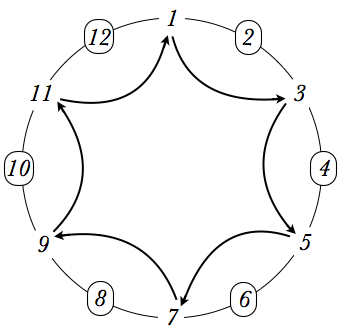
\includegraphics[scale=0.35]{FiguresMaths/josephus12step1}
        \hspace*{.2in}
        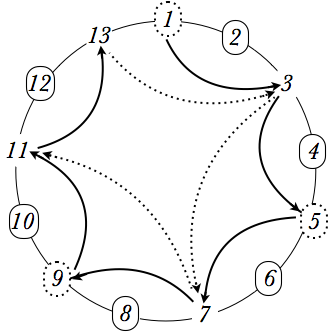
\includegraphics[scale=0.35]{FiguresMaths/josephus13}
\caption{(Left) First round of the Josephus erasure procedure for $n=12$.
(Right) First two rounds of the procedure when $n=13$; the first round is depicted by solid lines, the second by dotted lines. In both figures, the encircled integers are the ones that have been removed}
        \label{fig:josephus12step1}  \label{fig:josephus13}
\end{center}
\end{figure}

The following sequence of results provides a roadmap to the solution.

\medskip

We analyze \textit{rounds} of the process---sequences of elementary steps that return to the initial position, $1$.  If position $1$ has been erased, then its role is assumed by the then-smallest survivor.

\smallskip

Easily, the first round of the process takes $\lceil n/2 \rceil$ steps.  Each subsequent round then takes a number of steps that is ``half" the number of its preceding round.  We place ``half" in quotes to emphasize the required rounding-up of each halving.  

\medskip

Fig.~\ref{fig:josephus12step2}, which describes the final rounds of the process, lends intuition for the number of rounds before $J(n)$ stands alone.
\begin{figure}[ht]
\begin{center}
        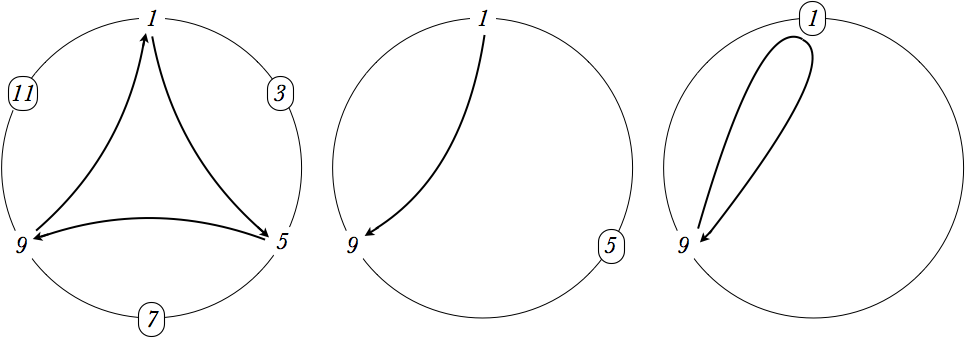
\includegraphics[scale=0.25]{FiguresMaths/josephus12LastSteps}
        \caption{The final rounds of the Josephus erasure process when $n=12$}
        \label{fig:josephus12step2}
\end{center}
\end{figure}

\medskip

The following four-part proposition now leads to the solution.

\begin{prop}
The value of $J(n)$, as determined by $n$:

\begin{tabular}{clll}
 & \underline{Condition on $n$} & \hspace*{.1in} & \underline{Value of $J(n)$} \\ 
{\bf (a)} &
For all $n$ &  & $J(n)$ is odd. \\
{\bf (b)} &
$n$ is even; i.e., $n = 2m$ & & $J(2m) \ = \ 2J(m)-1$ \\
{\bf (c)} &
$n$ is odd; i.e., $n = 2m+1$ & & $J(2m+1) = 2J(m)+1$ \\
{\bf (d)} &
$n = 2^m+k$, with $k < 2^m$ & & $J(2^m+k) = 2k+1$
\end{tabular}
\end{prop}

\ignore{************
\begin{proof}
This is a simple generalization of the previous proposition.  If $n$ is even, then the first round corresponds simply to come back to the original circle where one half of the points have been removed. 
\end{proof}

Next, grouping values of $n$ between successive powers of $2$, we find that

Let $n=2^m+k$, the rule within each group $m$ is to start at $1$ and increase by $2$ the successive numbers
($0 \leq k < 2^m$).
Let prove it by recurrence on $n$.
\medskip

\begin{prop}
For all $n = 2^m+k$, where $k < 2^m$, we have
$J(2^m+k) = 2k+1$.
\end{prop}

\begin{proof}
\begin{itemize}
\item {\bf Basis.} 
$n=1$, thus $m=0$, $k=0$ and $J(1) = 2^0+0 = 1$
\medskip\item {\bf Induction step.} 
Suppose the formula holds for any integer lower than $n=2^m+k$. 
Since there are two expressions for $J(.)$, we distinguish the cases whether $k$ is even or it is odd:
\begin{itemize}
\item If $k$ is even, then, $2^m+k$ is even, and we can write:

$J(2^m+k) = 2J(2^{m-1}+\frac{k}{2})-1$

by induction hypothesis, $J(2^{m-1} +\frac{k}{2}) = 2\frac{k}{2} +1 = k+1$

Thus, $J(2^m+k) = 2(k+1) -1 = 2k+1$.

\medskip\item If $k$ is odd, the proof is similar:

$J(2^m+k) = 2J(2^{m-1}+\lfloor \frac{k}{2} \rfloor)+1 = 2\lfloor \frac{k}{2} \rfloor +1 = 2k+1$.

\end{itemize}
\end{itemize}
\end{proof}
*****************}

\medskip

Your ultimate solution for $J(n)$ will emerge from analyzing what the preceding propositions yield as the value of $J(n)$.  

\smallskip

{\em Provide a closed-form expression for $J(n)$ in terms of $n$'s base-$2$ numeral.}
\medskip

{\em Hint.}
Consider the binary {\em numerals} for $n = 2^m +k$ and $k$.  We first note that, {\em numerically},
\begin{eqnarray*}
n & = &  2^m b_m \ + \ 2^{m-1} b_{m-1} \ + \cdots + \ 2 b_1 \ + \ b_0 \\
k & = & 2^{m-1}  b_{m-1} \ + \cdots + \ 2 b_1 \ + \ b_0
\end{eqnarray*} 
where each bit $b_i \in \{0,1\}$.  
%Therefore, in terms of {\em base-$2$ numerals}:
%\[ \begin{array}{ccrl}
%(n)_2 & = & 1 b_{m-1} \cdots b_1 b_0 & (\mbox{by definition, } \ b_m=1) \\ 
%(k)_2 & = & 0 b_{m-1} \cdots b_1 b_0 & (\mbox{because } [n = 2^m +k] \ \mbox{ and } \ k < 2^m)
%\end{array}
%\]

\ignore{*************
\[ (J(n))_2 \ = \ b_{m-1} \cdots b_0 b_m. \]
which indicates that $J(43) = 23$.  The pictorial interpretation of this coding is given in Fig.~\ref{fig:josephusCoding} for $n=43$.
\begin{figure}[h]
\begin{center}
        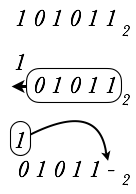
\includegraphics[scale=0.4]{FiguresMaths/josephusCoding}
        \caption{Obtaining the survivor number $J(43)$.}
        \label{fig:josephusCoding}
\end{center}
\end{figure}

The figure indicates that the solution for $J(n)$ is obtained by a simple shift of the binary representation of $n$.
**************}

\medskip\item
{\bf A ``trick'' for squaring integers whose decimal numeral ends in $5$}

{\sc Lesson:} Solving a fun problem by relating numbers to their numerals.

\smallskip

The uninitiated might misperceive the topic of this problem as an amusing ``trick''.  Of course, we would not present the ``trick" if there were not a serious mathematical message behind it.  Hopefully you will be inspired to design your own ``tricks". 

\medskip

Say that someone presents you with an integer $n$, by means of two-digit decimal numeral that ends in $5$.  You can compute $n^2$ virtually instantaneously.  

\smallskip

For instance: if someone says ``$n \ = \ 75$'',

\hspace{.25in}then you can instantly respond ``$n^2 \ = \ 5625$'';

if they say ``$m \ = \ 95$'',

\hspace{.25in}then you can instantly respond ``$m^2 \ = \ 9025$''.

\medskip

The ``trick" that leads to your responses underlies the following proposition.

\begin{prop}
\label{thm:square-(d5)}
If the integer $n$ has the decimal numeral $\delta 5$, where $\delta \in \{1, 2, \ldots, 9\}$, then 
\[ n^2 \ = \ 100 \times \delta \times (\delta+1) +25 \]
\end{prop}

(Note how our two examples satisfy this rule.)

\medskip

{\em Prove Proposition~\ref{thm:square-(d5)}.}

\smallskip

\textit{Hint.}
Review how numerals represent numbers.

\medskip\item
$\oplus \oplus$
{\bf An alternative to Horner's Rule}

{\sc Lesson:} Experience with operation-counting and asymptotics

\smallskip

In Section~\ref{sec:Horner-fast-evaluation}, we described Horner's Rule, a method for calculating polynomials faster than the common way of writing polynomials would suggest.  This exercise is devoted to an alternative streamlined polynomial evaluation procedure, called {\it Estrin's method}, after its inventor, Gerald Estrin \cite{Estrin60}.

\index{Estrin, Gerald} \index{Estrin's method (for evaluating univariate polynomials)}

\smallskip

Estrin's method begins with a polynomial of degree $d$ with real coefficients:
\[
P(x) \ \ = \ \ a_0 \ + \ a_1 x \ + \ a_2 x^2 \ + \cdots + \ a_{d-1} x^{d-1} \ + \ a_d x^d
\]
To avoid complicated expressions, we apply the method to the degree-$(d=7)$ polynomial:
\[
P_7(x) \ \ = \ \ a_0 \ + \ a_1 x \ + \ a_2 x^2 \ + \ a_3 x^3 \ + \ a_4 x^4 \ + \ a_5 x^5 \ + \ a_6 x^6 \ + \ a_7 x^7
\]

\smallskip

We begin by rewriting $P$ as follows, via repeated factorizations.
\[
P(x) \ \ = \ \ a_0 \ + \ x \cdot (a_1 \ + \ x \cdot (a_2  \ +  \cdots                                          
+ x \cdot (a_{d-2} \ + \ x \cdot (a_{d-1} \ + \ a_d x)) \cdots ))
\]
Applied to $P_7(x)$, this rewriting yields:
\[
P_7(x) \ \ = \ \ a_0 \ + \ a_1 x \ + \ x^2 \ ( a_2  \ + a_3 x \ ) \ + \ x^4 \ ( \ a_4 \ + \ a_5 x \ + \ x^2 \ ( a_6  \ + a_7 x \ ) \ )
\]
We then introduce the auxiliary recursive expressions.  
\begin{eqnarray*}
C_i^{(0)} & = & a_i + x a_{i+1} \\
                &\vdots &  \\
C_i^{(n)}  & = & C_i^{(n-1)} + x^{2n} C_{i+2^n}^{(n-1)}
\end{eqnarray*}
The method is completed by expressing $P(x)$ in terms of the auxiliary $C_i^{(k)}$

\smallskip

Example:
\begin{eqnarray*}
P_7(x) & = & C_{0}^{(0)} \ + \ x^2 \ C_2^{(0)} \ + \ x^4 \ ( \ C_4^{(0)} \ + \ x^2 \ C_6^{(0)} \ ) \\
            & = & C_0^{(1)} \ + \ x^4 \ C_4^{(1)}
\end{eqnarray*}

\medskip

{\em To do:}
\begin{enumerate}
\item
{\em Write $P(x)$ using the auxiliary expressions $C_i$.}  {\em To simplify this task, say that the degree $d$ is such that $d+1$ is a power of $2$.}
\medskip\item
{\em Determine how many additions and multiplications are required to evaluate $P(x)$.}
\end{enumerate}

\medskip\item
{\bf A simple, good, rational approximation to $e$}

{\sc Lesson:} Enhance understanding of the two main ways of representing rational numbers

\smallskip

It is well known that the decimal expansion of Euler's constant $e$ is infinite and non-periodic and that it begins
\[ e = 2.718281828 \cdots \]  
Therefore, Proposition~\ref{thm:rational-real} assures us that the infinite ultimately periodic decimal expansion (with added spaces to highlight the periodicity)
\[ 2.7 \ 1828 \ 1828 \ 1828 \ \cdots \ 1828 \ 1828 \ \cdots   \]
represents a rational number $r$ which agrees with $e$ for ten decimal places.

\smallskip

{\em Find a representation of $r$ as a fraction.  In more detail, find positive integers $p$ and $q$ such that}
\[ {p \over q} \ = \ r \ = \ 2.7 \ 1828 \ 1828 \ 1828 \ \cdots \ 1828 \ 1828 \ \cdots   \]


\medskip\item
$\oplus \oplus$ {\bf The uniqueness of Zeckendorf numerals}

{\sc Lesson:} Experience with Fibonacci numbers and with number representations

\smallskip

This problem refers to Zeckendorf numerals, which are representations of positive integers by sums of Fibonacci numbers.  The framework appears in detail in Section~\ref{sec:Fibo-numbers}.

\smallskip

{\em Prove that every positive integer has a unique Zeckendorf numeral}.

\end{enumerate}
